\documentclass[a4paper,11pt]{article}
\usepackage[T2A]{fontenc}     
\usepackage[utf8]{inputenc}  
\usepackage{lmodern}  
\usepackage{amsmath}
\usepackage{amsfonts}
\usepackage{amssymb} 
\usepackage{listings}
\usepackage{lstcustom}
\usepackage{graphicx}
\usepackage{geometry} % Меняем поля страницы
\geometry{left=2cm}% левое поле
\geometry{right=1.5cm}% правое поле
\geometry{top=1cm}% верхнее поле
\geometry{bottom=2cm}% нижнее поле



\renewcommand\contentsname{Содержание}
\renewcommand\partname{Часть}
\title{Лабораторная работа №1. Метод Гаусса с выбором главного элемента}
\author{Архангельский Илья}


\begin{document}
\begin{titlepage}
	\begin{center}
		БЕЛОРУССКИЙ ГОСУДАРСТВЕННЫЙ УНИВЕРСИТЕТ \\
		ФАКУЛЬТЕТ ПРИКЛАДНОЙ МАТЕМАТИКИ И ИНФОРМАТИКИ
	\end{center}
	\vspace{10em}
	\begin{center}
		\LARGE {Лабораторная работа \\
		по вычислительным методам алгебры на тему:}
		\linebreak	 
		
		Метод Гаусса с выбором главного элемента
	\end{center}
	\vspace{3em}
	\begin{flushright}
	  
	
 	Выполнил: \\	Архангельский И.А. \\ 
 	
 	  \vspace{1em}
 	
 	  Проверил: \\ Кондратюк А.П. \\
 	
	\end{flushright}
	
	\vfill
	\begin{center}
		Минск, 2012
	\end{center}
\end{titlepage} 

\newpage
\part{Входные и выходные данные.} 
\section*{Входные данные}
На \textbf{вход} программа принимает текстовый файл в котором первой строкой стоит целое неотрицательное число $n$, показывающее размерность матрицы $A$. Следующие $n$ строк содержат расширенную матрицу $[A|B]$. Где $B$ - столбец свободных членов.
\section*{Выходные данные}
На \textbf{выход}, в случае удачного решения СЛУ, в \textbf{stdout} выводится $x^T$, где $x$ - вектор-столбец, являющийся решением системы.  В случае, если систему решить невозможно, в \textbf{stdout} подается соответсвующая ошибка.
\newpage
\part{Блок-схема} 
\begin{figure}[h!]
\section*{Метод solve()}
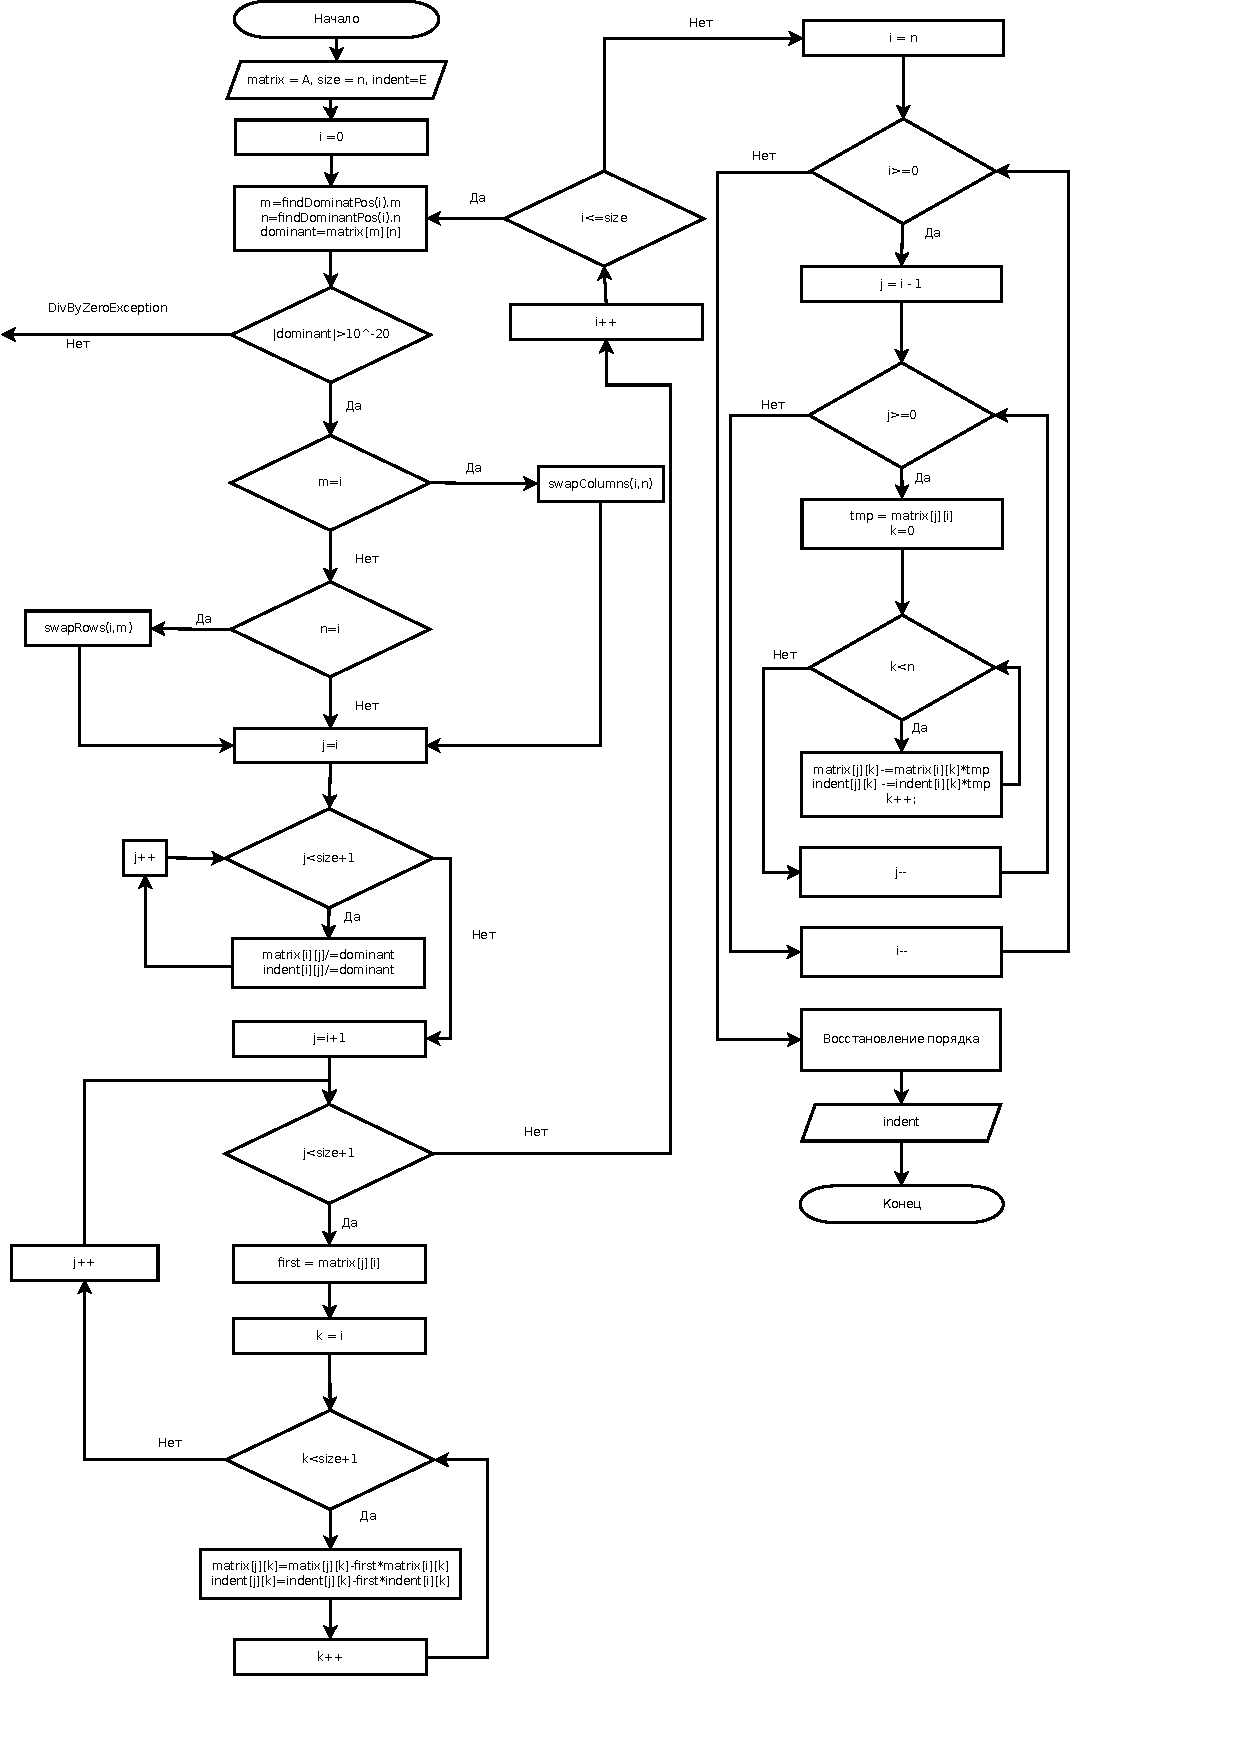
\includegraphics[scale=0.75]{flowchart1.pdf}
\end{figure}
\newpage
\section*{Вспомогательные методы}
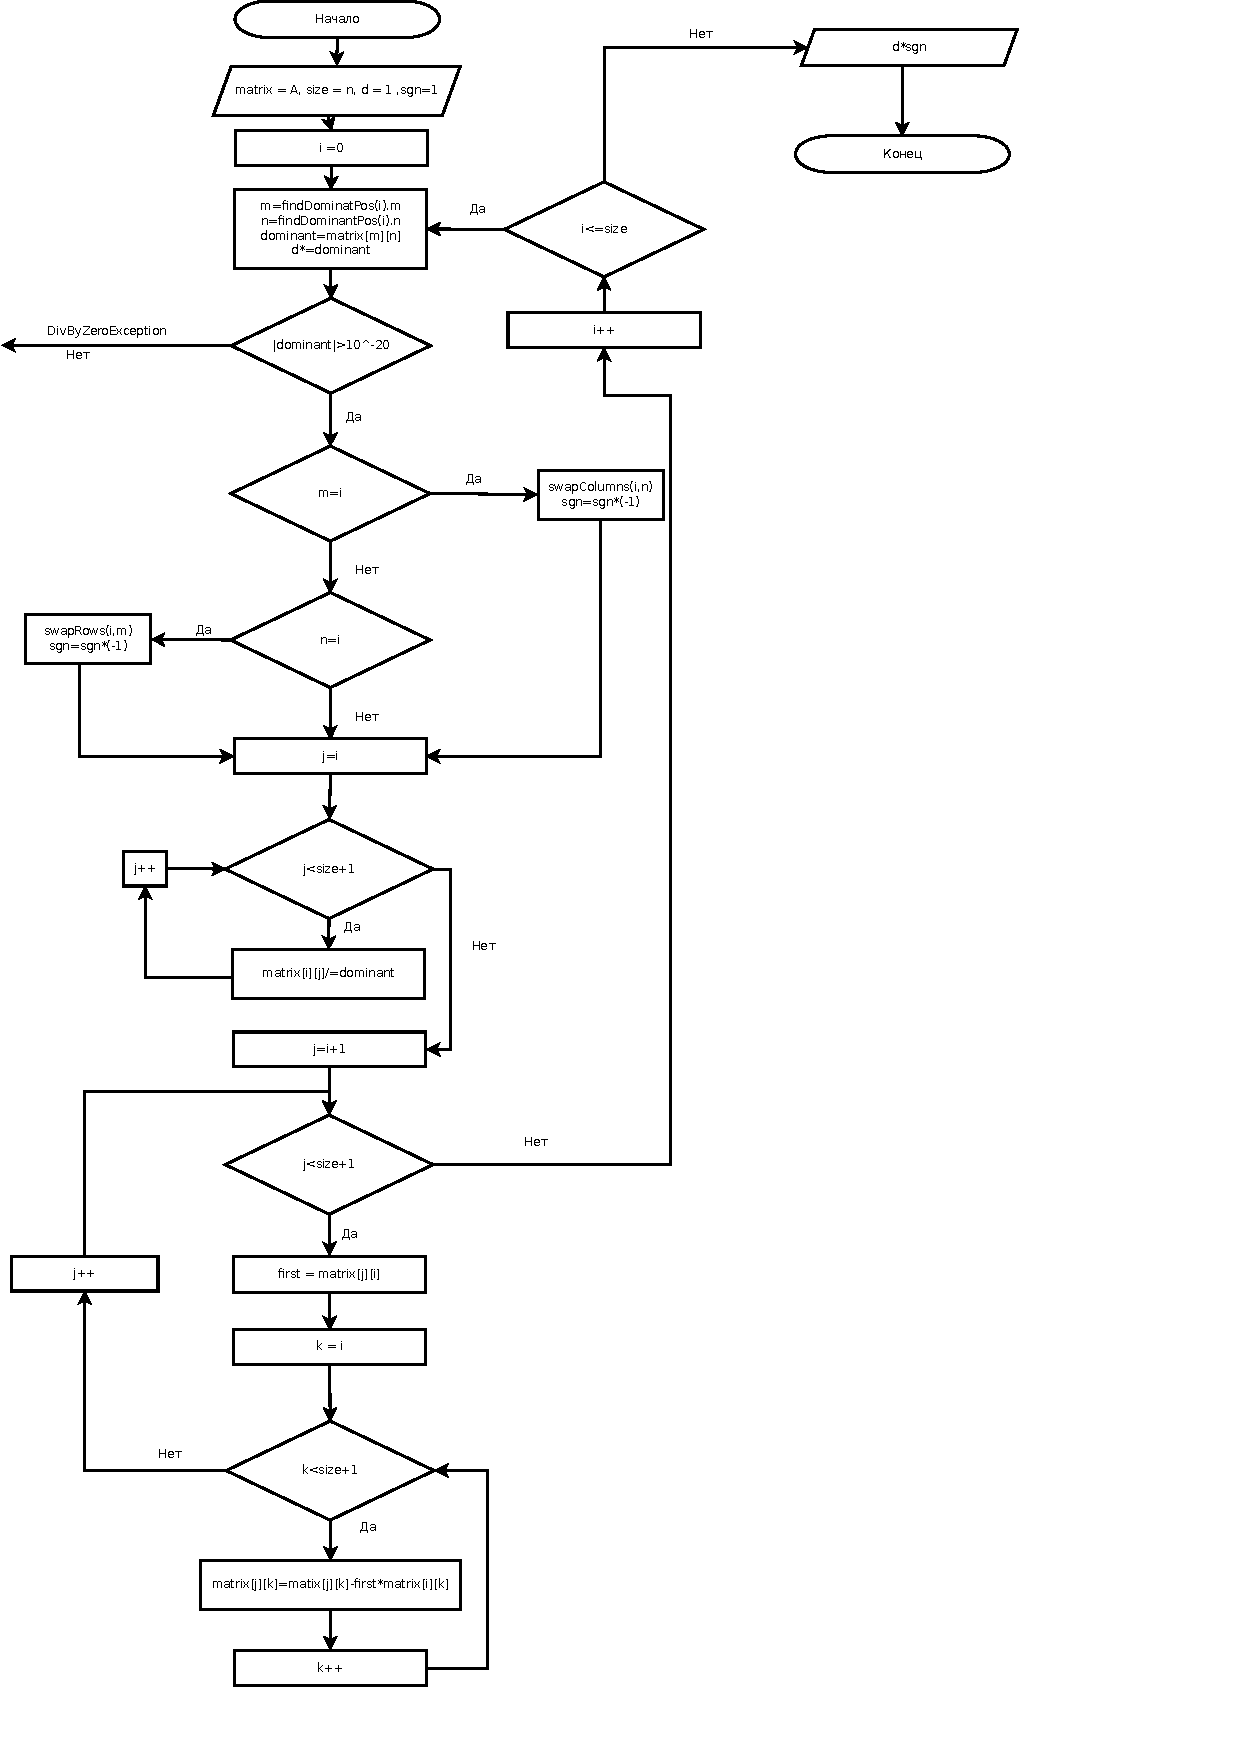
\includegraphics[width=\textwidth]{flowchart2.pdf}
 


\newpage
\part{Реализация}
\section*{gauss.h}
\begin{lstlisting} [language=c, style=eclipse]
#ifndef GAUSS_H
#define GAUSS_H

#include <cstdlib>
#include <stdio.h>
#include <math.h>
#include <iostream>

using namespace std;

struct DivByZeroException {};
struct CannotSolve {};
class Gauss
{
    double ** matrix;
    unsigned int size;
    int *permutation;

    struct Position
    {
        unsigned int n;
        unsigned int m;
    };

    void permutate (double* &x);
    Position findDominant (int k);
    void swapRows (int x, int y);
    void swapColumns (int x, int y);
public:
    Gauss(char* filename);
    double* solve ();
    int getSize() {return size;}
    ~Gauss ();
};

#endif // GAUSS_H

\end{lstlisting}
\newpage
\section*{gauss.cpp}
\begin{lstlisting}[language=c++, style=eclipse]
#include "gauss.h"

Gauss::Gauss (char *filename)
{
    FILE* fin = fopen (filename,"r");
    fscanf (fin,"%d\n",&size);
    matrix = new double* [size];
    for (int i=0;i<size;i++)
    {
        matrix[i]= new double [size+1];
        for (int j=0;j<size;j++)
        {
            fscanf(fin,"%lf",&matrix[i][j]);
        }
        fscanf (fin,"%lf\n",&matrix[i][size]);
    }
    permutation = new int [size];
    for (int i=0;i<size;i++)
    {
        permutation [i]= i;
    }
    fclose (fin);
}


Gauss::Position Gauss::findDominant(int k)
{
    Position pos;
    pos.m = k;
    pos.n = k;
    for (int i=k;k<size;k++)
    {
        if (fabs(matrix[i][k])>fabs(matrix[pos.m][pos.n]))
        {
            pos.m = i;
            pos.n = k;
        }
        if (fabs(matrix[k][i])>fabs(matrix[pos.m][pos.n]))
        {
            pos.m = k;
            pos.n = i;
        }
    }
    return pos;
}

void Gauss::swapRows(int x, int y)
{
    for (int i=1;i<size+1;i++)
    {
        double tmp = matrix[x][i];
        matrix [x][i] = matrix[y][i];
        matrix [y][i] = tmp;
    }
}

void Gauss::swapColumns(int x, int y)
{
    for (int i=0;i<size;i++)
    {
        double tmp = matrix[i][x];
        matrix [i][x] = matrix[i][y];
        matrix [i][y] = tmp;
    }
    int tmp = permutation[x];
    permutation [x] = permutation[y];
    permutation [y] = tmp;
}

double* Gauss::solve()
{
    for (int i=0;i<size;i++)
    {
        Position dominantPos = findDominant(i);
        double dominant = matrix[dominantPos.m][dominantPos.n];
        if (fabs(dominant)<pow(10,-20)) throw DivByZeroException ();
        if (dominantPos.m==i)
        {
            swapColumns(i,dominantPos.n);
        }
        if (dominantPos.n==i)
        {
            swapRows(i,dominantPos.m);
        }

        for (int j=i;j<size+1;j++)
        {
            matrix[i][j]/=dominant;
        }

        for (int j=i+1;j<size;j++)
        {
            double first = matrix[j][i];
            for (int k=i;k<size+1;k++)
            {
                matrix[j][k]=matrix[j][k] - first*matrix[i][k];
            }
        }
    }

    double* X = new double [size];
    for (int i=size-1;i>-1;i--)
    {
        double x = matrix[i][size];
        for (int j=i+1;j<size;j++)
        {
            x -= matrix[i][j]*X[j];
        }
        if (matrix[i][i]==0)
        {
            throw CannotSolve();
        }
        X[i]=x/matrix[i][i];
    }
    permutate (X);

    return X;
}

void Gauss::permutate(double *&x)
{
    double* res = new double [size];
    for (int i=0;i<size;i++)
    {
        res[permutation[i]]=x[i];
    }
    for (int i=0;i<size;i++)
    {
        x[i]=res[i];
    }
    delete res;
}

Gauss::~Gauss()
{
    for (int i=0;i<size;i++)
    {
        delete matrix[i];
    }
    delete matrix;
    delete permutation;
}
\end{lstlisting}
\newpage
\section*{main.cpp}
\begin{lstlisting}[language=c++, style=eclipse]
#include <cstdlib>
#include <iostream>
#include "gauss.h"

using namespace std;

int main(int argc, char *argv[])
{
    for (int i=1;i<argc;i++)
    {
        Gauss gauss =  Gauss(argv[1]);
        double * res = NULL;
        try
        {
            res = gauss.solve();
        }
        catch (DivByZeroException e)
        {
            printf ("ERR::DIVIZION BY ZERO\n");
            continue;
        }
        catch (CannotSolve e)
        {
            printf ("ERR::Something got wrong.Can't solve this.\n");
            continue;
        }

        printf ("RUNNING ON TEST: %s\n",argv[i]);
        for (int i=0;i<gauss.getSize();i++)
        {
            printf ("%8.3lf  ",res[i]);
        }
        printf ("\n");
        delete res;
    }
    return 0;

}
\end{lstlisting}
\newpage
\part{Тестовые данные}
\begin{footnotesize}
\section{Тест}
\subsection*{01.in}
\begin{lstlisting}
4
3 8 3 -1 4
2 3 4 1 -4
1 -3 -2 -2 3
5 -8 4 2 -8  
\end{lstlisting}
\subsection*{stdout}
\begin{lstlisting}
RUNNING ON TEST: 01.in
   2.000     1.000    -3.000     1.000 
\end{lstlisting}
\section{Тест}

\subsection*{03.in}
\begin{lstlisting}
3
0 0 0 0 
0 0 0 0
0 0 0 0
\end{lstlisting}
\subsection*{stdout}
\begin{lstlisting}
RUNNING ON TEST: 03.in
ERR::DIVIZION BY ZERO
\end{lstlisting}
\section{Тест}
\subsection*{04.in}
\begin{lstlisting}
3
1 1 1 1
1 1 0 2
1 2 3 0
\end{lstlisting}
\subsection*{stdout}
\begin{lstlisting}
RUNNING ON TEST: 04.in
   1.000     1.000    -1.000   
\end{lstlisting}
\section{Тест}
\subsection*{05.in}
\begin{lstlisting}
2
30 30 60
30 30 0
\end{lstlisting}

\subsection*{stdout}
\begin{lstlisting}
RUNNING ON TEST: 05.in
ERR::DIVIZION BY ZERO
\end{lstlisting}
\end{footnotesize}
\end{document}
